\documentclass[TFM.tex]{subfiles}

\begin{document}


\chapter{Formality of Chain Operad of Little Disks}\label{4}



%EN GENERAL LO QUE PUEDA DE TAMARKIN
%
%
%\url{https://ncatlab.org/nlab/show/augmentation}
%
%\url{https://ncatlab.org/nlab/show/Drinfeld+associator}


In this chapter we review and explain the heart of the proof of the Deligne Conjecture: the formality of the chain operad of little disks. Throughout this chapter we follow \cite{Tamarkin}. The chain operad of little disks is the operad of chain complexes over $\Q$ obtained from the topological little disks operad. By formailty it is meant that this operad is equivalent to its homology operad in the sense that there is a \emph{zig-zag} of quasi-isomorphisms (i.e. maps inducing isomorphisms on homology) between them. The strategy is the following:

 First, we define an operad which is homotopy equivalent to the little disks operad from a category operad $PaB_*$. Then, we take a $\Q$-linear span of $PaB_*$ and find an operad $O_A(*)$ together with a quasi-isomorphism from the homology operad of little disks. Finally, we give a quasi-isomorphism between the span $\Q(PaB_*)$ and $O_A(*)$, which completes the proof. 




\section{Braided operads and little disks operads}

We can substitute the group $\Sigma_n$ in the definition \ref{operadtop} by the braid group $B_n$, since there is a projection $B_n\to \Sigma_n$ with kernel $PB_n$ assigning to each braid $\sigma\in B_n$ the permutation that it induces on its endpoints. This way we obtain the notion of \emph{braided operad}. A \emph{topological $B_\infty$-operad} $X$ is defined to be a braided operad such that all its spaces $X(n)$ are contractible and the braid group $B_n$ acts freely on $X(n)$. If $X$ and $Y$ are topological $B_\infty$-operads, then so is $X\times Y$ in an obvious way and we have homotopy equivalences 
\begin{equation}\label{projections}
p_1:X\times Y\to X;\ p_2:X\times Y\to Y,
\end{equation}
where $p_1$, $p_2$ are the projections. 

Given a topological $B_\infty$-operad $X$, the corresponding \emph{operad of little disks} is a symmetric operad $X'$ such that $X'(n)=X(n)/PB_n$ with the induced structure maps. Since the maps in \ref{projections} and their homotopy inverses are $PB_n$-equivariant, any two operads of little disks are connected by a chain of homotopy equivalences, because the equivalence $X\simeq Y$ induces a well-defined homotopy equivalence $X/PB_n\simeq Y/PB_n$. 

%We require in addition that the actions are nice enough so that the maps $X(n)\to X'(n)$ are covering maps. This way, $X'(n)$ is a $K(PB_n,1)$ space, so any two operads of little disks are homotopy equivalent. Using the maps \ref{projections} we can explicitly connect any two operads of little disks by a chain of homotopy equivalences. The projection $X×Y→X$ is $PB_n$-equivariant at each level for the product action on $(X\times Y)(n)=X(n)×Y(n)$ and so induces a map $X(n)×Y(n)/PB_n→X/PB_n$. This map is a fiber bundle with fiber $Y(n)$ (it is trivialized over any open subset of $X(n)/PB_n$ that is evenly covered by $X(n)→X(n)/PB_n$) and thus a homotopy equivalence since $Y(n)$ is contractible. Similarly, the other projection gives a homotopy equivalence $X(n)×Y(n)/PB_n→Y(n)/PB_n$ and combining them we get a homotopy equivalence $X(n)/PB_n→Y(n)/PB_n$.


We now prove that the little disks operad defined in Section \ref{little} is a little disks operad in this sense. We'll make use of the following lemmas.

\begin{lemma}\label{contractible}
Let $(X,A)$ be a pair of topological spaces where $A$ is a contractible subspace  and let $p:\widetilde{X}\to X$ be a covering map. Then $p^{-1}(A)$ is a disjoint union of subspaces of $\widetilde{X}$, each of them mapped homeomorphically onto $A$ by $p$. 
\end{lemma}
\begin{proof}
In general, a fibre bundle over a contractible space is trivial \cite[Proposition 3.5]{bundle}, meaning that $p_X^{-1}(A)\cong A\times F_{x}$, where $F_x$ is the fibre over any point of $x\in A$. Since $p_X$ is a covering map, this fiber is discrete and we are done. 
\end{proof}

\begin{lemma}\label{lift}
Under the conditions of the previous leema, assume chosen base points $x\in A$ of $X$ and $y=f(x)\in B$ of $Y$ and choose lifts $\widetilde{A}$ of $A$ and $\widetilde{B}$ of $B$ given by the previous lemma. Choose also lifts $\widetilde{x}\in\widetilde{A}$ of $x$ and $\widetilde{y}\in\widetilde{B}$ of $y$. Then, if $f$ lifts to $\widetilde{f}:(\widetilde{X},\widetilde{x})\to (\widetilde{Y},\widetilde{y})$ as a map of based spaces, then $f$ lifts to $\widetilde{f}:(\widetilde{X},\widetilde{A})\to (\widetilde{Y},\widetilde{B})$ as a map of pairs. 
\end{lemma}
\begin{proof}
Since $A$ is contractible, it is path-connected, and so is $\widetilde{A}$. Then $\widetilde{f}(A)$ is a connected subspace of $\widetilde{Y}$ containing $\widetilde{y}$. Moreover, $p_Y(\widetilde{f}(A)(=f(p_X(\widetilde{A}))=f(A)$, so $\widetilde{f}(\widetilde{A})$ is contained in $p_Y^{-1}(B)$, more specifically in the connected component containing $\widetilde{y}$, which is $\widetilde{B}$. Hence, $\widetilde{f}$ is actually a map of pairs.
\end{proof}

Now we follow the example 3.1 of \cite{bar} to prove:

\begin{prop}
The operad $E_2$ defined in Section \ref{little} is a little disks operad in the sense described above.
\end{prop} 
\begin{proof}
Let $\widetilde{E}_2(n)$ denote the universal cover of $E_2(n)$. We will dfine
an operad structure and braid group actions on $\widetilde{E}_2$ by lifting them from the
structure map and symmetric group actions on $E_2$. Let $p:\widetilde{E}_2\to E_2$ the universal covering and let $E_1\subseteq E_2$ be the ``horizontal'' embedding of $E_1$ as little cubes of the form

\definecolor{xdxdff}{rgb}{0.49019607843137253,0.49019607843137253,1.}
\begin{tikzpicture}[line cap=round,line join=round,>=triangle 45,x=1.0cm,y=1.0cm]
\clip(-3.5866666666666673,-0.4666666666666) rectangle (11.293333333333335,4.5);
\fill[line width=2.pt,color=xdxdff,fill=xdxdff,fill opacity=0.10000000149011612] (0.41333333333333344,4.) -- (0.4,0.) -- (0.7733333333333334,0.) -- (0.7866666666666668,4.) -- cycle;
\fill[line width=2.pt,color=xdxdff,fill=xdxdff,fill opacity=0.10000000149011612] (1.2,4.) -- (1.2133333333333338,0.) -- (1.586666666666667,0.) -- (1.586666666666667,4.) -- cycle;
\fill[line width=2.pt,color=xdxdff,fill=xdxdff,fill opacity=0.10000000149011612] (3.,4.) -- (3.,0.) -- (3.386666666666667,0.) -- (3.4,4.) -- cycle;
\draw[line width=2.pt] (0.41333333333333344,4.) -- (0.4,0.) -- (0.7733333333333334,0.) -- (0.7866666666666668,4.) -- cycle;
\draw[line width=2.pt] (1.2,4.) -- (1.2133333333333338,0.) -- (1.586666666666667,0.) -- (1.586666666666667,4.) -- cycle;
\draw[line width=2.pt] (3.,4.) -- (3.,0.) -- (3.386666666666667,0.) -- (3.4,4.) -- cycle;
\draw [line width=2.pt] (0.,0.)-- (0.,4.);
\draw [line width=2.pt] (0.,4.)-- (4.,4.);
\draw [line width=2.pt] (4.,4.)-- (4.,0.);
\draw [line width=2.pt] (4.,0.)-- (0.,0.);
\draw [line width=2.pt,color=xdxdff] (0.41333333333333344,4.)-- (0.4,0.);
\draw [line width=2.pt,color=xdxdff] (0.4,0.)-- (0.7733333333333334,0.);
\draw [line width=2.pt,color=xdxdff] (0.7733333333333334,0.)-- (0.7866666666666668,4.);
\draw [line width=2.pt,color=xdxdff] (0.7866666666666668,4.)-- (0.41333333333333344,4.);
\draw [line width=2.pt,color=xdxdff] (1.2,4.)-- (1.2133333333333338,0.);
\draw [line width=2.pt,color=xdxdff] (1.2133333333333338,0.)-- (1.586666666666667,0.);
\draw [line width=2.pt,color=xdxdff] (1.586666666666667,0.)-- (1.586666666666667,4.);
\draw [line width=2.pt,color=xdxdff] (1.586666666666667,4.)-- (1.2,4.);
\draw [line width=2.pt,color=xdxdff] (3.,4.)-- (3.,0.);
\draw [line width=2.pt,color=xdxdff] (3.,0.)-- (3.386666666666667,0.);
\draw [line width=2.pt,color=xdxdff] (3.386666666666667,0.)-- (3.4,4.);
\draw [line width=2.pt,color=xdxdff] (3.4,4.)-- (3.,4.);
\draw [line width=2.pt] (0.41333333333333344,4.)-- (0.4,0.);
\draw [line width=2.pt] (0.4,0.)-- (0.7733333333333334,0.);
\draw [line width=2.pt] (0.7733333333333334,0.)-- (0.7866666666666668,4.);
\draw [line width=2.pt] (0.7866666666666668,4.)-- (0.41333333333333344,4.);
\draw [line width=2.pt] (1.2,4.)-- (1.2133333333333338,0.);
\draw [line width=2.pt] (1.2133333333333338,0.)-- (1.586666666666667,0.);
\draw [line width=2.pt] (1.586666666666667,0.)-- (1.586666666666667,4.);
\draw [line width=2.pt] (1.586666666666667,4.)-- (1.2,4.);
\draw [line width=2.pt] (3.,4.)-- (3.,0.);
\draw [line width=2.pt] (3.,0.)-- (3.386666666666667,0.);
\draw [line width=2.pt] (3.386666666666667,0.)-- (3.4,4.);
\draw [line width=2.pt] (3.4,4.)-- (3.,4.);
\draw (0.35,2.38) node[anchor=north west] {$1$};
\draw (1.15,2.38) node[anchor=north west] {$2$};
\draw (2.95,2.38) node[anchor=north west] {$n$};
\draw (1.9,2.353333333333338) node[anchor=north west] {$\cdots$};
\end{tikzpicture}

ordered from left to right as shown. Note that the little squares are homotopy equivalent to the little disks. Choose the non-$\Sigma$ version of $E_1$ as ``base contractible space'' (as in \ref{contractible}) and call it again $E_1$. By lemma \ref{contractible} and the fact that $E_1$ is contractible (see Section \ref{intervals}, Proposition \ref{E1}) we have that $p^{-1}(E_1(n))\subseteq\widetilde{E}_2(n)$ is a disjoint union of components, each homeomorphic to $E_1(n)$ via $p$. For each $n$, arbitrarily choose one these components and call it $\widetilde{E}_1(n)$. 

Now define the structure map $\widetilde{\gamma}$ for $\widetilde{E}_2$ to be the unique lifting 
\[
\begin{tikzcd}
\widetilde{E}_2(k)\times\widetilde{E}_2(j_1)\times\cdots\widetilde{E}_2(j_k) \arrow[r, "\widetilde{\gamma}", dashed] \arrow[d, "p"] & \widetilde{E}_2(j_1+\cdots+j_k) \arrow[d, "p"] \arrow[d] \\
E_2(k)\times E_2(j_1)\times\cdots E_2(j_1+\cdots+j_k) \arrow[r, "\gamma"]                                                                      & E_2(j_1+\cdots+j_k)                                     
\end{tikzcd}
\]
which takes $\widetilde{E}_1(k)\times\widetilde{E}_1(j_1)\times\cdots\widetilde{E}_1(j_k)$ to $\widetilde{E}_1(j_1+\cdots+j_k)$. The existence and uniqueness of this map is guaranteed by lemma \ref{lift} since $\gamma$ clearly takes the embedding $E_1(k)\times E_1(j_1)\times\cdots E_1(j_k)$ to the embedding of $E_1(j_1+\cdots+j_k)$. Here we're implicitly making use of the theory of covering spaces, in particular the lifting properties of the universal cover (see Section 1.3 of \cite{Hatcher} for a complete treatment of the subject). Also recall that the product of covering spaces is a covering space of the product (Exercise 2 from page 79 of \cite{Hatcher}).

Finally we have to define the braid group actions $\widetilde{E}_2(n)\times B_n\to\widetilde{E}_2(n)$. It suffices
to specify actions by the standard generators $\widetilde{\sigma}_i$, $1 \leq i \leq n - 1$, where $\widetilde{\sigma}_i$ denotes
the braid

\begin{figure}[h!]
\centering
\begin{tikzpicture}

\braid[ number of strands=12, %lower bound
 border height=2pt,style strands={10}{line width=2pt}, style strands={9}{draw=none},style strands={8}{line width=2pt},style strands={7}{line width=2pt},style strands={6}{line width=2pt},style strands={5}{line width=2pt}, style strands={4}{draw=none},style strands={3}{line width=2pt}, style strands={11,1,2,12}{draw=none}] (braid) at (1,0)%optional, it's a name
         a_{11} a_6 a_{11};
           \node[ at=(braid-3-s),  label=north :  $1$ ] {} ;
          \node[ at=(braid-6-s),  label=north :  $i$ ] {} ;
\node[ at=(braid-7-s),  label=north : $i+1$ ] {} ;
\node[ at=(braid-10-s),  label=north :  $n$ ] {} ;
%\draw (6.5,-2) node[anchor=south] {$\sigma_i$};
\fill[black] ( 8.7 , -1.5 ) circle ( 1 pt ) ;
\fill[black] ( 9 , -1.5 ) circle ( 1 pt ) ;
\fill[black] ( 9.3 , -1.5 ) circle ( 1 pt ) ;

\fill[black] ( 3.7 , -1.5 ) circle ( 1 pt ) ;
\fill[black] ( 4 , -1.5 ) circle ( 1 pt ) ;
\fill[black] ( 4.3 , -1.5 ) circle ( 1 pt ) ;
\end{tikzpicture}
\end{figure}

%suces

%Si defino la composición operádica como la única que hace conmutar el diagrama de recubrimientos entonces necesariamente es morfismo de operads
We will specify the action by this braid to be the lift of the action of $\sigma_i = (i\ i+1)\in\Sigma_n$ on $E_2(n)$ subject to the following basepoint condition. %CREO QUE LA IDEA ES QUE LA ACCIÓN SIEMPRE LIFTEA PERO DEPENDE DE LA ELECCIÓN DE PUNTO BASE, SI NO ME ACLARO ESTO PREGUNTARLE A MURO PORQUE AQUÍ NO SE DEFINE LA ACCIÓN EN TODO EL RECUBRIDOR, SOLO EN EL LIFT DE $E_1$ 
Choose an arbitrary point $x\in E_1(n)$. Let $\alpha:I\to E_2(n)$ denote the path from $x$ to $x\sigma_i$ specified by the following sequence
of pictures

\definecolor{qqqqff}{rgb}{0.,0.,1.}
\resizebox{13cm}{9.8cm}{%
\begin{tikzpicture}[line cap=round,line join=round,>=triangle 45,x=1.0cm,y=1.0cm]
\clip(-3.8,-6.1) rectangle (13.293333333333337,5.7);
\fill[line width=2.pt,color=qqqqff,fill=qqqqff,fill opacity=0.10000000149011612] (0.37333333333333335,5.) -- (0.7733333333333334,5.) -- (0.8,0.) -- (0.4,0.) -- cycle;
\fill[line width=2.pt,color=qqqqff,fill=qqqqff,fill opacity=0.10000000149011612] (1.6,5.) -- (2.186666666666667,5.) -- (2.2,0.) -- (1.6133333333333333,0.) -- cycle;
\fill[line width=2.pt,color=qqqqff,fill=qqqqff,fill opacity=0.10000000149011612] (2.6133333333333333,5.) -- (3.3866666666666667,5.) -- (3.4133333333333336,0.) -- (2.6,0.) -- cycle;
\fill[line width=2.pt,color=qqqqff,fill=qqqqff,fill opacity=0.10000000149011612] (4.2,5.) -- (4.613333333333333,5.) -- (4.626666666666667,0.) -- (4.226666666666667,0.) -- cycle;
\fill[line width=2.pt,color=qqqqff,fill=qqqqff,fill opacity=0.10000000149011612] (6.4,5.) -- (6.4,0.) -- (6.786666666666667,0.) -- (6.8,5.) -- cycle;
\fill[line width=2.pt,color=qqqqff,fill=qqqqff,fill opacity=0.10000000149011612] (10.626666666666667,5.) -- (10.626666666666667,0.) -- (10.2,0.) -- (10.24,5.) -- cycle;
\fill[line width=2.pt,color=qqqqff,fill=qqqqff,fill opacity=0.10000000149011612] (7.626666666666667,0.) -- (7.613333333333334,2.393333333333333) -- (8.213333333333335,2.4066666666666663) -- (8.213333333333335,0.) -- cycle;
\fill[line width=2.pt,color=qqqqff,fill=qqqqff,fill opacity=0.10000000149011612] (8.613333333333333,5.) -- (8.6,2.58) -- (9.4,2.58) -- (9.426666666666668,5.) -- cycle;
\fill[line width=2.pt,color=qqqqff,fill=qqqqff,fill opacity=0.10000000149011612] (0.4,-1.) -- (0.4133333333333334,-6.) -- (0.8,-6.) -- (0.8,-1.) -- cycle;
\fill[line width=2.pt,color=qqqqff,fill=qqqqff,fill opacity=0.10000000149011612] (4.613333333333333,-6.) -- (4.613333333333333,-1.) -- (4.2,-1.) -- (4.226666666666667,-6.) -- cycle;
\fill[line width=2.pt,color=qqqqff,fill=qqqqff,fill opacity=0.10000000149011612] (1.6133333333333333,-1.) -- (1.6133333333333335,-3.406666666666663) -- (2.4,-3.406666666666663) -- (2.4,-1.) -- cycle;
\fill[line width=2.pt,color=qqqqff,fill=qqqqff,fill opacity=0.10000000149011612] (2.8,-6.) -- (2.8133333333333335,-3.606666666666663) -- (3.4,-3.606666666666663) -- (3.413333333333334,-6.) -- cycle;
\fill[line width=2.pt,color=qqqqff,fill=qqqqff,fill opacity=0.10000000149011612] (6.373333333333334,-1.) -- (6.4,-6.) -- (6.8,-6.) -- (6.8133333333333335,-1.) -- cycle;
\fill[line width=2.pt,color=qqqqff,fill=qqqqff,fill opacity=0.10000000149011612] (10.6,-6.) -- (10.6,-1.) -- (10.2,-1.) -- (10.213333333333335,-6.) -- cycle;
\fill[line width=2.pt,color=qqqqff,fill=qqqqff,fill opacity=0.10000000149011612] (8.386666666666667,-1.) -- (8.413333333333334,-6.) -- (7.613333333333334,-6.) -- (7.6,-1.) -- cycle;
\fill[line width=2.pt,color=qqqqff,fill=qqqqff,fill opacity=0.10000000149011612] (8.813333333333334,-1.) -- (8.8,-6.) -- (9.4,-6.) -- (9.413333333333334,-1.) -- cycle;
\draw [line width=2.pt] (0.,0.)-- (0.,5.);
\draw [line width=2.pt] (0.,5.)-- (5.,5.);
\draw [line width=2.pt] (5.,5.)-- (5.,0.);
\draw [line width=2.pt] (5.,0.)-- (0.,0.);
\draw [line width=2.pt] (6.,0.)-- (6.,5.);
\draw [line width=2.pt] (6.,5.)-- (11.,5.);
\draw [line width=2.pt] (11.,5.)-- (11.,0.);
\draw [line width=2.pt] (11.,0.)-- (6.,0.);
\draw [line width=2.pt] (0.,-1.)-- (0.,-6.);
\draw [line width=2.pt] (0.,-6.)-- (5.,-6.);
\draw [line width=2.pt] (5.,-6.)-- (5.,-1.);
\draw [line width=2.pt] (5.,-1.)-- (0.,-1.);
\draw [line width=2.pt] (6.,-1.)-- (11.,-1.);
\draw [line width=2.pt] (11.,-1.)-- (11.,-6.);
\draw [line width=2.pt] (11.,-6.)-- (6.,-6.);
\draw [line width=2.pt] (6.,-6.)-- (6.,-1.);
\draw [line width=2.pt] (0.37333333333333335,5.)-- (0.4,0.);
\draw [line width=2.pt] (0.7733333333333334,5.)-- (0.8,0.);
\draw [line width=2.pt] (1.6,5.)-- (1.6133333333333333,0.);
\draw [line width=2.pt] (2.186666666666667,5.)-- (2.2,0.);
\draw [line width=2.pt] (2.6133333333333333,5.)-- (2.6,0.);
\draw [line width=2.pt] (3.3866666666666667,5.)-- (3.4133333333333336,0.);
\draw [line width=2.pt] (4.613333333333333,5.)-- (4.626666666666667,0.);
\draw [line width=2.pt] (4.2,5.)-- (4.226666666666667,0.);
\draw [line width=2.pt,color=qqqqff] (6.4,5.)-- (6.4,0.);
\draw [line width=2.pt,color=qqqqff] (6.4,0.)-- (6.786666666666667,0.);
\draw [line width=2.pt,color=qqqqff] (6.786666666666667,0.)-- (6.8,5.);
\draw [line width=2.pt,color=qqqqff] (6.8,5.)-- (6.4,5.);
\draw [line width=2.pt,color=qqqqff] (10.626666666666667,5.)-- (10.626666666666667,0.);
\draw [line width=2.pt,color=qqqqff] (10.626666666666667,0.)-- (10.2,0.);
\draw [line width=2.pt,color=qqqqff] (10.2,0.)-- (10.24,5.);
\draw [line width=2.pt,color=qqqqff] (10.24,5.)-- (10.626666666666667,5.);
\draw [line width=2.pt,color=qqqqff] (7.626666666666667,0.)-- (7.613333333333334,2.393333333333333);
\draw [line width=2.pt,color=qqqqff] (7.613333333333334,2.393333333333333)-- (8.213333333333335,2.4066666666666663);
\draw [line width=2.pt,color=qqqqff] (8.213333333333335,2.4066666666666663)-- (8.213333333333335,0.);
\draw [line width=2.pt,color=qqqqff] (8.213333333333335,0.)-- (7.626666666666667,0.);
\draw [line width=2.pt,color=qqqqff] (8.613333333333333,5.)-- (8.6,2.58);
\draw [line width=2.pt,color=qqqqff] (8.6,2.58)-- (9.4,2.58);
\draw [line width=2.pt,color=qqqqff] (9.4,2.58)-- (9.426666666666668,5.);
\draw [line width=2.pt,color=qqqqff] (9.426666666666668,5.)-- (8.613333333333333,5.);
\draw [line width=2.pt,color=qqqqff] (0.4,-1.)-- (0.4133333333333334,-6.);
\draw [line width=2.pt,color=qqqqff] (0.4133333333333334,-6.)-- (0.8,-6.);
\draw [line width=2.pt,color=qqqqff] (0.8,-6.)-- (0.8,-1.);
\draw [line width=2.pt,color=qqqqff] (0.8,-1.)-- (0.4,-1.);
\draw [line width=2.pt,color=qqqqff] (4.613333333333333,-6.)-- (4.613333333333333,-1.);
\draw [line width=2.pt,color=qqqqff] (4.613333333333333,-1.)-- (4.2,-1.);
\draw [line width=2.pt,color=qqqqff] (4.2,-1.)-- (4.226666666666667,-6.);
\draw [line width=2.pt,color=qqqqff] (4.226666666666667,-6.)-- (4.613333333333333,-6.);
\draw [line width=2.pt,color=qqqqff] (1.6133333333333333,-1.)-- (1.6133333333333335,-3.406666666666663);
\draw [line width=2.pt,color=qqqqff] (1.6133333333333335,-3.406666666666663)-- (2.4,-3.406666666666663);
\draw [line width=2.pt,color=qqqqff] (2.4,-3.406666666666663)-- (2.4,-1.);
\draw [line width=2.pt,color=qqqqff] (2.4,-1.)-- (1.6133333333333333,-1.);
\draw [line width=2.pt,color=qqqqff] (2.8,-6.)-- (2.8133333333333335,-3.606666666666663);
\draw [line width=2.pt,color=qqqqff] (2.8133333333333335,-3.606666666666663)-- (3.4,-3.606666666666663);
\draw [line width=2.pt,color=qqqqff] (3.4,-3.606666666666663)-- (3.413333333333334,-6.);
\draw [line width=2.pt,color=qqqqff] (3.413333333333334,-6.)-- (2.8,-6.);
\draw [line width=2.pt,color=qqqqff] (6.373333333333334,-1.)-- (6.4,-6.);
\draw [line width=2.pt,color=qqqqff] (6.4,-6.)-- (6.8,-6.);
\draw [line width=2.pt,color=qqqqff] (6.8,-6.)-- (6.8133333333333335,-1.);
\draw [line width=2.pt,color=qqqqff] (6.8133333333333335,-1.)-- (6.373333333333334,-1.);
\draw [line width=2.pt,color=qqqqff] (10.6,-6.)-- (10.6,-1.);
\draw [line width=2.pt,color=qqqqff] (10.6,-1.)-- (10.2,-1.);
\draw [line width=2.pt,color=qqqqff] (10.2,-1.)-- (10.213333333333335,-6.);
\draw [line width=2.pt,color=qqqqff] (10.213333333333335,-6.)-- (10.6,-6.);
\draw [line width=2.pt,color=qqqqff] (8.386666666666667,-1.)-- (8.413333333333334,-6.);
\draw [line width=2.pt,color=qqqqff] (8.413333333333334,-6.)-- (7.613333333333334,-6.);
\draw [line width=2.pt,color=qqqqff] (7.613333333333334,-6.)-- (7.6,-1.);
\draw [line width=2.pt,color=qqqqff] (7.6,-1.)-- (8.386666666666667,-1.);
\draw [line width=2.pt,color=qqqqff] (8.813333333333334,-1.)-- (8.8,-6.);
\draw [line width=2.pt,color=qqqqff] (8.8,-6.)-- (9.4,-6.);
\draw [line width=2.pt,color=qqqqff] (9.4,-6.)-- (9.413333333333334,-1.);
\draw [line width=2.pt,color=qqqqff] (9.413333333333334,-1.)-- (8.813333333333334,-1.);
\draw [line width=2.pt] (6.4,5.)-- (6.8,5.);
\draw [line width=2.pt] (6.4,5.)-- (6.4,0.);
\draw [line width=2.pt] (6.4,0.)-- (6.786666666666667,0.);
\draw [line width=2.pt] (6.786666666666667,0.)-- (6.8,5.);
\draw [line width=2.pt] (7.613333333333334,2.393333333333333)-- (8.213333333333335,2.4066666666666663);
\draw [line width=2.pt] (8.213333333333335,2.4066666666666663)-- (8.213333333333335,0.);
\draw [line width=2.pt] (7.613333333333334,2.393333333333333)-- (7.626666666666667,0.);
\draw [line width=2.pt] (7.626666666666667,0.)-- (8.213333333333335,0.);
\draw [line width=2.pt] (8.613333333333333,5.)-- (9.426666666666668,5.);
\draw [line width=2.pt] (9.426666666666668,5.)-- (9.4,2.58);
\draw [line width=2.pt] (9.4,2.58)-- (8.6,2.58);
\draw [line width=2.pt] (8.6,2.58)-- (8.613333333333333,5.);
\draw [line width=2.pt] (10.24,5.)-- (10.2,0.);
\draw [line width=2.pt] (10.2,0.)-- (10.626666666666667,0.);
\draw [line width=2.pt] (10.626666666666667,0.)-- (10.626666666666667,5.);
\draw [line width=2.pt] (10.626666666666667,5.)-- (10.24,5.);
\draw [line width=2.pt] (0.4,-1.)-- (0.8,-1.);
\draw [line width=2.pt] (0.8,-1.)-- (0.8,-6.);
\draw [line width=2.pt] (0.8,-6.)-- (0.4133333333333334,-6.);
\draw [line width=2.pt] (0.4133333333333334,-6.)-- (0.4,-1.);
\draw [line width=2.pt] (1.6133333333333333,-1.)-- (1.6133333333333335,-3.406666666666663);
\draw [line width=2.pt] (1.6133333333333335,-3.406666666666663)-- (2.4,-3.406666666666663);
\draw [line width=2.pt] (2.4,-3.406666666666663)-- (2.4,-1.);
\draw [line width=2.pt] (2.4,-1.)-- (1.6133333333333333,-1.);
\draw [line width=2.pt] (2.8133333333333335,-3.606666666666663)-- (3.4,-3.606666666666663);
\draw [line width=2.pt] (3.413333333333334,-6.)-- (3.4,-3.606666666666663);
\draw [line width=2.pt] (2.8133333333333335,-3.606666666666663)-- (2.8,-6.);
\draw [line width=2.pt] (2.8,-6.)-- (3.413333333333334,-6.);
\draw [line width=2.pt] (4.226666666666667,-6.)-- (4.2,-1.);
\draw [line width=2.pt] (4.613333333333333,-1.)-- (4.613333333333333,-6.);
\draw [line width=2.pt] (4.613333333333333,-6.)-- (4.226666666666667,-6.);
\draw [line width=2.pt] (4.2,-1.)-- (4.613333333333333,-1.);
\draw [line width=2.pt] (6.373333333333334,-1.)-- (6.4,-6.);
\draw [line width=2.pt] (6.4,-6.)-- (6.8,-6.);
\draw [line width=2.pt] (6.8,-6.)-- (6.8133333333333335,-1.);
\draw [line width=2.pt] (6.8133333333333335,-1.)-- (6.373333333333334,-1.);
\draw [line width=2.pt] (7.6,-1.)-- (7.613333333333334,-6.);
\draw [line width=2.pt] (7.613333333333334,-6.)-- (8.413333333333334,-6.);
\draw [line width=2.pt] (8.413333333333334,-6.)-- (8.386666666666667,-1.);
\draw [line width=2.pt] (8.386666666666667,-1.)-- (7.6,-1.);
\draw [line width=2.pt] (8.813333333333334,-1.)-- (8.8,-6.);
\draw [line width=2.pt] (8.8,-6.)-- (9.4,-6.);
\draw [line width=2.pt] (9.4,-6.)-- (9.413333333333334,-1.);
\draw [line width=2.pt] (9.413333333333334,-1.)-- (8.813333333333334,-1.);
\draw [line width=2.pt] (10.2,-1.)-- (10.213333333333335,-6.);
\draw [line width=2.pt] (10.213333333333335,-6.)-- (10.6,-6.);
\draw [line width=2.pt] (10.6,-6.)-- (10.6,-1.);
\draw [line width=2.pt] (10.6,-1.)-- (10.2,-1.);
\draw (0.4,2.6) node[anchor=north west] {$1$};
\draw (1.72,2.6) node[anchor=north west] {$i$};
\draw (0.9,2.5) node[anchor=north west] {$\cdots$};
\draw (2.5,2.6) node[anchor=north west] {\small{$i+1$}};
\draw (3.4,2.5) node[anchor=north west] {$\cdots$};
\draw (4.2,2.6) node[anchor=north west] {$n$};
\draw (6.4,2.6) node[anchor=north west] {$1$};
\draw (7.72,2.193333333333332) node[anchor=north west] {$i$};
\draw (8.5,4.393333333333331) node[anchor=north west] {\small{$i+1$}};
\draw (6.9,2.5) node[anchor=north west] {$\cdots$};
\draw (9.4,2.5) node[anchor=north west] {$\cdots$};
\draw (0.4,-2.9) node[anchor=north west] {$1$};
\draw (1.5,-2.) node[anchor=north west] {\small{$i+1$}};
\draw (2.9,-4.38) node[anchor=north west] {$i$};
\draw (4.2,-2.9) node[anchor=north west] {$n$};
\draw (6.4,-2.9) node[anchor=north west] {$1$};
\draw (0.8,-3.) node[anchor=north west] {$\cdots$};
\draw (3.493333333333334,-3.0) node[anchor=north west] {$\cdots$};
\draw (6.8,-3.) node[anchor=north west] {$\cdots$};
\draw (7.5,-2.9) node[anchor=north west] {\small{$i+1$}};
\draw (8.95,-2.9) node[anchor=north west] {$i$};
\draw (9.48,-3.) node[anchor=north west] {$\cdots$};
\draw (10.15,-2.9) node[anchor=north west] {$n$};
\draw (10.2,2.6) node[anchor=north west] {$n$};
\end{tikzpicture}
}\\

Let $\widetilde{\alpha}$ denote the lift which starts in $\widetilde{C}_1$. Let $\widetilde{x}=\widetilde{\alpha}(0)$ and $\widetilde{y}=\widetilde{\alpha}(1)$, then specify $\widetilde{x}\widetilde{\sigma}=\widetilde{y}$. %COMPROBAR QUE ESTO DA LA ESTRUCTURA DE $B_\infty$ (ADEMÁS DE LAS PROPIEDADES DE OPERAD, LA ACCIÓN TIENE QUE SER LIBRE, PERO TENGO DUDA PARA EL CASO DE LAS TRENZAS PURAS) Y QUE EL COCIENTE POR LA ACCIÓN DE LAS TRENZAS PURAS ES $E_2$ (QUIZÁ ESTO SEA PORQUE PRECISAMENTE ES EL GRUPO FUNDAMENTAL, PERO TENGO QUE REVISAR SI ES LA MISMA ACCIÓN QUE LA DEL GRUPO FUNDAMENTAL)
This data specifies a $B_\infty$-operad structure on $\widetilde{E}_2$. 
%EL EJEMPLO DE FIEDEROWICZ CON LA PRUEBA DEL EJERCICO QUE ME PUSO MURO (A infinito significa que los espacios del operad son contráctiles, esto para el caso sin acción del grupo simétrico, que es el que usa Fiedorowicz. Con acción significa que cada componente conexa es contráctil, pero en cualquier caso C1 es contráctil \url{https://en.wikipedia.org/wiki/A\%E2\%88\%9E-operad}) 
\end{proof}

A more general approach to the previous proposition is taken in propositions 2.27 and 2.28 of \cite{tesis}

We now give a few useful definitions from \cite[\textsection 2.6]{Kontsevich}. Let $P$ be an operad of complexes (dg-operad), and $f : A→B$ be a morphism of two $P$-algebras.
\begin{defi}
$f$ is a quasi-isomorphism if it induces an isomorphism of the homology
groups of $A$ and $B$ considered as complexes with zero differential.
\end{defi}

\begin{defi}
Two algebras $A$ and $B$ are called \emph{homotopy equivalent} if there exists a chain (or zig-zag) of quasi-isomorphisms
\[
A= A_1→A_2←A_3→\cdots←A_{2k+1} = B
\]
\end{defi}

Analogously to the case of algebras, we can speak about quasi-isomorphisms of operads
of complexes.

\begin{defi}
A morphism $f : P_1→P_2$ between two dg-operads is called a
\emph{quasi-isomorphism} if the maps of chain complexes $f(n) : P_1(n)→P_2(n)$ induce isomorphisms of
homology groups for all $n$.
\end{defi}

\begin{defi}
Two dg-operads $A$ and $B$ are said to be \emph{equivalent} if there exists a chain of quasi-isomorphisms
\[
A= A_1→A_2←A_3→\cdots←A_{2k+1} = B
\]
\end{defi}


The functor of singular chains $C_*^{sing}:\Top\to \Ch$ has a natural tensor (lax monoidal) structure given by the Eilenberg-Zilber map $EZ:C_*^{sing}(X)\otimes C_*^{sing}(Y)\to C_*^{sing}(X\times Y)$ as we saw in section \ref{zilber} of chapter \ref{3}. Therefore, for a topological operad $O$, the coleccion $C_*^{sin}(O(*))$ has a structure of a dg-operad. The structure map of the $i$-th insertion is 
\[
C_*^{sing}(O(n))\otimes C_*^{sing}(O(m))\xrightarrow{EZ} C_*^{sing}(O(n)\times O(m))\xrightarrow{\circ_{i*}} C_*^{sing}(O(n+m-1)),
\]
where $\circ_i$ is the structure map of the $i$-th insertion in $O$. 

For a little disks operad $X$ consider the operad $C_2(X)=C_*^{sing}(X)$. Any two such operads are quasi-isomorphic. In particular, the homology operad of any $C_2(X)$ is the operad $e_2=H_*(E_2)$ controlling Gerstenhaber algebras. Our goal in this chapter is to show the following.

\begin{thm}
Any operad $C_2(X)$ is equivalent to its homology operad $e_2$.
\end{thm}

It suffices to prove this theorem only for one operad $X$ of little disks since they are all homotopy equivalent. We will prove it for the one defined in the next section.

\section{The category operad $PaB_n$}\label{pab}

We're going to define a category operad $PaB_n$. Let $B_n$ the group of braids on $n$ strands and $PB_n$ the group of pure braids on $n$ strand. Let $\Sigma_n$ the symmetric group and let $p:B_n\to \Sigma_n$ be the canonical projection with kernel $PB_n$. We assume that the strands of any braid are numbered in the order determined by their origins. We also need to add the grous $B_0=B_1=1$.

The objects of the category $PaB_n$ are parenthesized permutations of the set $\{1,\dots, n\}$ (that is pairs $(\sigma,\pi)$, where $\sigma\in\Sigma_n$ and $\pi$ is a parenthesizing of the non-associative product of $n$ elements). The morphisms between $(\sigma_1,\pi_1)$ and $(\sigma_2,\pi_2)$ are such braids in $B_n$ that any strand joins an element of $\sigma_1$ with the same element of $\sigma_2$, in other words, $\Hom((\sigma_1,\pi_1),(\sigma_2,\pi_2))=p^{-1}(\sigma_2^{-1}\sigma_1)$. The composition law is induced from the one on $B_n$. The symmetric group $\Sigma_n$ acts on $PaB_n$ via renumbering the objects: $\tau(\sigma,\pi)=(\tau\sigma,\pi)$ for $\tau\in\Sigma_n$ and $(\sigma,\pi)\in PaB_n$. 

%\url{https://ncatlab.org/nlab/show/parenthesized+braid+operad}

The collection of categories $PaB_n$ form an operad. Indeed, the collection of objects $PaB_*$ forms an operad in the category of magmas (sets generated by one non-commutative operation). The insertion at the level of objects can be described as follows. Consider two permutations $\sigma_p\in\Sigma_p$ and $\sigma_q\in\Sigma_q$. To perform the $i$-th insertion ($1\leq i\leq p$) of $\sigma_q$ in $\sigma_p$, the set $\{1,\dots, q\}$ must be inserted in the set $\{1,\dots, i,\dots, p\}$ to get the set $\{1,\dots, i,\dots,i+q-1,\dots, p+q-1\}$. Then, the permutation $\sigma_{p+q-1}\in\Sigma_{p+q-1}$ is obtained by applying $\sigma_p$ on the latter set, acting on the block $\{i,\dots, p+q-1\}$ as if it were only one element sent to the position $\sigma_p(i)$, and then permuting that block using $\sigma_q$. The parenthesizing is the obvious one. 

Let us describe the structre map $\circ_k$ of the insertion into the $k$-th position on the level of morphisms. Suppose we insert $y:(\sigma_1,\pi_1)\to (\sigma_2,\pi_2)$ into $x:(\sigma_3,\pi_3)\to(\sigma_4,\pi_4)$. We replace the strand number $\sigma^{-1}_3(k)$ of the braid $x$ by the braid $y$ made very narrow, as shown in the picture.

\begin{figure}[h!]
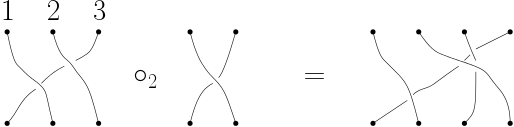
\includegraphics[scale=0.7]{Imagenes/insercion.png}
\caption{Insertion of the right braid into the second strand of the left braid.}
\end{figure}
\subsection{Operations on $PaB_n$}\label{operations}
There are a few operations on $PaB_*$ that will be useful later and that can be found in Section 2 of \cite{1deTamarkin}, but adopting the convention that the strands of the braids are parametrized from bottom to top. These are operations on the morphism, so they are operations on each braid group $B_n$. Let $B\in B_n$, then the operations are the following.

\begin{itemize}
	\item  \emph{Extension operations}: let $d_0B = d^n_0	B$ ($d_{n+1}B = d^n_{n+1}B$) be $B$ with one straight strand
	added on the left (right), with ends regarded as outer-most:
	\begin{figure}[h!]
		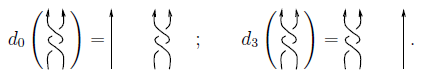
\includegraphics[scale=0.5]{Imagenes/extension}
	\end{figure}
	
	\item \emph{Cabling operations}: let $d_iB = d^n_i B$ for $1 ≤ i ≤ n$ be the parenthesized braid obtained
from $B$ by doubling its $i$-th strand (counting at the top):
\begin{figure}[h!]
		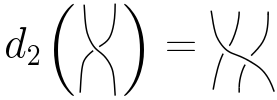
\includegraphics[scale=0.5]{Imagenes/cabling}
	\end{figure}
	
	\item \emph{Strand removal operations}: Let $s_iB = s^n_i B$ for $1 ≤ i ≤ n$ be the parenthesized braid
obtained from $B$ by removing its $i$-th strand (counting at the top):
	\begin{figure}[h!]
		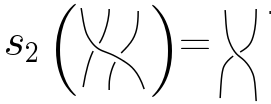
\includegraphics[scale=0.5]{Imagenes/removal}
	\end{figure}
	
\end{itemize}

\subsection{Operad of classifying spaces}

We have the functor of taking the nerve $N:\Cat\to\SSet$ and the functor of topological realization $|\ |:\SSet\to \CW$. One can easily check that the nerve functor behaves well with respect to the symmetric monoidal structure. Since the nerve of $PaB_n$ is countable, the realization also behaves well with its symmetric monoidal structure by \ref{countable}. Therefore the collection of cellular complexes $X_n=|N(PaB_n)|$ forms a cellular operad. Let us check that this operad is a little disks operad. Let $PaB_n'$ be the category whose objects are pairs $(x,y)$, where $x$ belongs to the braid group $B_n$ and $y$ is a parenthesizing of the non-associative product of $n$ elements, and there is a unique morphism between any two objects. We have a free left action of $B_n$ on $PaB_n':(x,y)\to (gx,y)$ and a braided operad structre on $PaB_*'$ (the structre maps are defined similarly to $PaB_n$). We have to show that the corresponding operad of classifying spaces is a topological $B_\infty$-operad and that the corresponding little disks operad is isomorphic to $X_*$. The action of $B_n$ on $PaB_n'$ induces an action on the vertices (0-simplices) of $|N(PaB_n')|$ and can be extended linearly to the whole complex, and therefore it is automatically free. Then, the quotient $|N(PaB_n')|/PB_n$ is equivalent to $X_n$ since the morphisms $(\sigma_1,\pi_1)\to(\sigma_2,\pi_2)$ in $PaB_n$ can be obtained by choosing one element in $p^{-1}(\sigma_2^{-1}\sigma_1)$ and multiplying it by the elements of $PB_n$. %NO ESTOY SEGURO DE QUE ESTÉ BIEN ESTO QUE HE DICHO.

Consider the corresponding chain operad. Let $C_*(PaB_n)$ be the chain complex over $\Q$ of $NPaB_n$ as a simplicial set. The collection $C_*(PaB_n)$ forms a dg-operad (via the Eilenberg-Zilber map). 

We have a canonical quasi-isomorphism of operads $C_*(PaB_*)\to C_*^{sing}(|NPaB_*|)$ (just like the quasi-isomorphism between simplicial homology and singular homology, see \cite[\textsection 2.1]{Hatcher}). Therefore it suffices to construct a quasi-isomorphism of $C_*(PaB_*)$ and $e_2$.

\section{Operad $O_A(*)$ and construction of a quasi-isomorphisms}

Let $A_n$ be the algebra over $\Q$ of power series in the noncommutative variables $t_{ij}$, where $i\geq 1$, $j\leq n$, $i\neq j$ and $t_{ij}=t_{ji}$, with relations $[t_{ij}+t_{ik},t_{kj}]=0$. This algebra is defined in \cite{Tamarkin} and in \cite{1deTamarkin}. Let $I_n$ be the two-sided ideal generated by all $t_{ij}$. We have a canonical projection 
\begin{equation}\label{canonical}
\pi:A_n\to A_n/I_n\cong\Q.
\end{equation}
The symmetric group $\Sigma_n$ acts naturally on $A_n$ via $\sigma\cdot t_{ij}=t_{\sigma(i)\sigma(j)}$. The collection $\{A_n\}_{n\geq 0}$ (being $A_0$ trivial) forms an operad of algebras as we shall see. The map of the insertion into the $i$-th position $\circ_i: A_n\otimes A_m\to A_{n+m-1}$ looks as follows. Define
\[
\phi(k)=\begin{cases}
k, & k\leq i;\\
k+m-1, & k>i.
\end{cases}
\]
Then, the insertion into the $i$-th position is the linear extension of
\begin{align*}
&o_i(t_{pq}\otimes 1)=\begin{cases}
t_{\phi(p)\phi(q)}, &p,q\neq i;\\
\sum_{r=i}^{i+m-1}t_{r\phi(q)}, & p=i.
\end{cases} \\
& o_i(1\otimes t_{pq})=t_{i+p-1,i+q-1}
\end{align*}
One can verify that this map satisfies the expected properties of the operadic composition. %DEBERÍA 

Any algebra with unit over $\Q$, say $A$, gives rise to a $\Q$-additive category $C_A$ with one object. Denote by $\Q\Cat$ the category of all small $\Q$-additive categories, and by $\Q\Cat'=\Q\Cat/C_\Q$ the slice category of $\Q\Cat$ over $C_\Q$. The objects of $\Q\Cat'$ are the elements of $\Hom(x, C_\Q)$ for each $x\in \Q\Cat'$. A morphism between $\varphi:x\to C_\Q$ and $\psi:y\to C_\Q$ is a morphism $\eta: x\to y$ in $\Q\Cat$ such that $\eta\psi=\varphi$.  This category has a clear symmetric monoidal structure obtained by the usual one on $\Cat$. We have the functor of nerve
$N^{\Q}: \Q\Cat'\to \SVect$, which is analogue to nerve of an arbitrary
category (but with slight nuances that we will detail soon), and the functor $C_*: \SVect \to\Ch$ of chain complexes over $\Q$. Both of these functors are lax monoidal (on the latter functor it is defined via the Eilenberg–Zilber map), therefore we have a functor $\Q\Cat'\to\Ch$ and the induced functor $C_*^{\Q}:\Q\Cat'$-Operads $\to$ dg-Operads. 
%CREO QUE DEBO PREGUNTAR CÓMO SE DEFINE EL COMPLEJO DE CADENAS DE UN OBJETO SIMPLICIAL \url{https://ncatlab.org/nlab/show/Dold-Kan+correspondence} SEGURAMENTE ES PONER CADA NIVEL COMO COMPONENTE Y HACER LA TÍPICA SUMA ALTERNADA CON LAS CARAS PARA LA DIFERENCIAL

The map (\ref{canonical}) produces a morphism $\pi_*: C_{A_n}\to C_\Q$ and defines an object
$O_A(n)\in \Q\Cat'$. The operad structure on $A_n$ defines an operad structure on the
collection $\{O_A(n)\}$. 
%En los racionales es la identidad porque solo se defien cuando hay algún t, así que pasa como slice. Tal como está definida la inserción se puede entender además desde el producto cartesiano y se puede trasladar al producto en Cat
To see what the complex $C_*^{\Q}(O_A(n))$ looks like, we explain how the $\Q$-linear nerve functor $N^\Q$ works. For the usual nerve $N$ acting on a category $\CC$, the set of $n$-simplices can be written as
\[
\coprod_{x_1,\dots, x_n\in\mathrm{Ob}\CC}\CC(x_2,x_1)\times\cdots \times\CC(x_{n+1},x_{n})
\]
where $\CC(x_{i+1},x_i)=\Hom_{\CC}(x_{i+1},x_i)$. Since we are in a linear context, we can replace disjoint unions by direct sums and cartesian products by tensor products. In each coordinate of the direct sum, we have elements of the form
\[
f_1\otimes\cdots \otimes f_{n}
\]
with $f_i\in \CC(x_{i+1},x_i)$. In particular, when $\CC$ has only one object, these are indeed the $n$-simplices. For $1<i<n$, the face maps are straight analogues to the general case, i.e. $$d_i(f_1\otimes\cdots \otimes f_{i-1}\otimes f_i\otimes \cdots\otimes f_n)=f_1\otimes\cdots \otimes f_{i-1}f_i\otimes\cdots \otimes f_n$$
For $i=1,n$, we need to modify the face maps, since omitting $f_1$ or $f_n$ doesn't yield a homomorphism (because projections are not bilinear). Instead, we define
\[
d_1(f_1\otimes f_2\otimes\cdots\otimes f_n)=g(f_1)f_2\otimes\cdots\otimes f_n
\]
and
\[
d_n(f_1\otimes\cdots\otimes f_{n-1}\otimes f_n)=f_1\otimes\cdots\otimes f_{n-1} g(f_n),
\]
where $g$ is a linear map which can be chosen depending on the context. Generally, $g$ is chosen not to be the identity because in that case $d_1=d_2$ and $d_{n-1}=d_n$. 
%NO ME PARECE NADA EVIDENTE QUE SALGA LO QUE PONE A CONTINUACIÓN A PARTIR DE LA CONSTRUCCIÓN DEL ANTERIOR PÁRRAFO. 

Thus, the complex $C_*^{\Q}(O_A(n))$ looks as follows. The degree $k$ component $C_k^{\Q}(O_A(n))$ is $A_n^{\otimes k}$ and the differential is given by %CREO QUE ES PORQUE CADA ESPACIO VECTORIAL SIMPLICIAL ESTÁ GENERADO POR CADENAS DE MORFISMOS DE LONGITUD FIJA, QUE ES LO MISMO QUE COGER TUPLAS and the boundary map is given by
\[
d(a_1\otimes\cdots\otimes a_n)=\pi(a_1)a_2\otimes\cdots\otimes a_n-a_1a_2\otimes \cdots\otimes a_n+\cdots+(-1)^{n}a_1\otimes\cdots\otimes a_{n-1}\pi(a_n)
\]
%COMPROBAR QUE SIN METERLE EL PI EN MEDIO VALE, PERO DE TODAS FORMAS CONSULTAR
\subsection{Construction of quasi-isomorphisms}
Let $e_2$ be the operad of graded vector spaces governing the Gerstenhaber algebras.
It is generated by two binary operations: the commutative associative multiplication of degree zero, which is denoted by $\cdot$, and the commutative bracket of degree 1 denoted by $[,]$. 

These operations satisfy the Leibniz identity
\[
[ab, c]= a[b, c]+(-1)^{|b|(|c|+1)}[a,c]b
\]
and the Jacoby identity
\[
(-1)^{(|a|-1)(|c|-1)}[[a,b],c]+(-1)^{(|b|-1)(|a|-1)}[[b,c],a]+(-1)^{(|c|-1)(|b|-1)}[[c,a],b]=0.
\]
We have a morphism of operads
\[
h:e_2\to C_*^{\Q}(O_A)
\]
which is defined on $e_2(2)$ as follows:
\[
h(\mu)=1\in C_0^\Q(O_A),\ h(l)=t_{12}\in C_1^\Q(O_A),
\]

where $\mu(a,b)=a\cdot b$ and $l(a,b)=(-1)^{|a|}[a,b]$. To see that this map is well defined, we shall interpret the properties of the product and the Lie bracket in terms of element of the operads. Since both $\mu$ and $l$ are operations in arity 2, we have two insertion maps $\circ_1$, $\circ_2$ corresponding to introducing an element in the first or the second argument respectively. The action of the symmetric group consists of rearranging the arguments according to each permutation.

Now, commutativity of $\mu$ can be expressed as $\mu=(12)\mu$, since $\mu(a,b)=(-1)^{|a||b|}\mu(b,a)$, and by the Koszul sign convention, that sign is equivalent to permute $a$ and $b$, so we can write $\mu(a,b)=\mu(12)(a,b)$, which is what we wrote at the beginning.  Associativity can be expressed simply as $\mu\circ_1\mu=\mu\circ_2\mu$.

Similarly, we have 
\[
l(a,b)=-(-1)^{(|a|-1)(|b|-1)+|a|+|b|}l(b,a)=(-1)^{|a||b|}l(b,a)=l(12)(a,b),
\]
so $l=(12)l$. Now, let us transcript the Leibniz identity into the operadic language. We have, 
\[
(-1)^{|a|+|b|}l(\mu(a,b),c)=\mu((-1)^{|a|+|b|}\mu(a,(-1)^{|b|}l(b,c))+(-1)^{|b|(|c|+1)}\mu((-1)^{|a|}l(a,c),b)
\]
which rewrites in terms of operadic composition, using that $|l|=1$ for the signs, as %la a salta sobre l y por eso sale el signo |a|*1, no salta sin embargo sobre (b,c), es decir, tienes l b c y saltas solo l, por eso el signo no es a(b+c-1)
\[
(-1)^{|a|+|b|}(l\circ_1\mu)(a,b,c)=(-1)^{|a|+|b|}\mu\circ_2 l(a,b,c)+(-1)^{|b|(|c|+1)+|a|+|b||c|}(23)\mu\circ_1 l(a,b,c).
\]
The signs cancel, so we can simplify this as
\[
l\circ_1\mu =\mu\circ_2 l +(23)\mu\circ_1 l.
\]

Finally, let us rewrite the Jacobi identity. Recall that $|[a,b]|=|a|+|b|-1$, so the Jacobi identity is
\begin{gather*}
(-1)^{(|a|-1)(|c|-1)+|a|+|b|-1+|a|}l\circ_1 l(a,b,c)+(-1)^{(|b|-1)(|c|-1)+|b|+|c|-1+|b|+|a|(|b|+|c|)}l\circ_1 l(132)(a,b,c)+\\
+(-1)^{(|c|-1)(|b|-1)+|c|+|a|-1+|c|+|c|(|a|+|b|)}l\circ_1 l(123)(a,b,c)=0.
\end{gather*}
After computing the signs, one sees that they are all equal to $(-1)^{|a||c|+|a|+|b|+|c|}$, so the equation simplyfies to
\[
l\circ_1 l+(132)l\circ_1 l+(123)l\circ_1 l=0
\]

Having this relations, direct check shows that the map $h$ respects them. 

%CREO QUE $t_{12}$ ES EL PRODUCTO POR ESTE ELEMENTO, YA QUE YENDO ATRÁS SE ESTÁ VIENDO EL ÁLGEBRA COMO UNA CATEGORÍA, PERO EN ESE CASO DEBERÍA ESPECIFICAR SI ES A IZQUIERDA O A DERECHA (QUIZÁ SOLO UNA CUMPLA LAS CONDICIONES, ASÍ QUE INTENTAR COMPROBARLO), AUN ASÍ ESTÁ MANDANDO OPERACIONES BINARIAS A OPERACIONES UNARIAS, NO LE VEO SENTIDO. Direct check shows that this map respects the relations in $e_2$ COMPROBAR.
%
%NO ENTIENDO LO QUE ME HA PEDIDO FERNANDO, AUNQUE PARA EMPEZAR NO ENTIENDO LO DE QUE EL OPERAD ESTÉ GENERADO POR ESAS OPERACIONES, CUANDO ESAS OPERACIONES SON DEL ÁLGEBRA, NO DEL OPERAD (SERÁ QUE ES UN ÁLGEBRA SOBRE SÍ MISMA). LUEGO, TENDRÍA QUE VERIFICAR QUE LAS RELACIONES DE ESTAS OPERACIONES SE VERIFICAN CON EL 1 Y EL T12 DE LA LLEGADA. NO SÉ PARA QUÉ ES LO DE EXPRESARLAS EN TÉRMINOS OPERÁDICOS NI CÓMO SE HACE, PORQUE ESTABA MEZCLANDO MU CON LA INSERCCIÓN, PERO SE SUPONE QUE MU ES YA UNA INSERCIÓN O NO SÉ (CREO QUE NO TENGO QUE PENSAR QUE ES UNA INSERCIÓN, SINO QUE ES SIMPLEMENTE UN PRODUCTO, QUE PARTE DE AxA Y LUEGO LA INSERCIÓN METE OTRA COPIA DE A (AUNQUE SI QUIERO HACERLA CON MU NECESITO 2), PARA LO CUAL SE PUEDE USAR LA ASOCIATIVIDAD. PERO SI ENTIENDES LA ANTICONMUTATIVIDAD DE LIE COMO ACCIÓN DE UNA TRASPOSICIÓN, ENTONCES NO PUEDES MANDARLO A T12 PORQUE ES SIMÉTRICO CON RESPECTO A ESA ACCIÓN, ADEMÁS SI LO INTERPRETO COMO OPERACIÓN DE OPERAD LA ASOCIATIVIDAD ME DARÍA QUE ES ASOCIATIVO
%
%ME RALLA QUE LA ARIDAD LA DE EL SUBÍNDICE Y NO EL NÚMERO DE COPIAS DEL ÁLGEBRA
%
%POSIBLEMENTE SE REFIERE A LA OPERACIÓN DEL OPERAD DE HOMOLOGÍA, PERO TENGO QUE PREGUNTAR IGUALMENTE LO DE QUE ESTE ESTÉ GENERADO POR ESO, QUE NO SÉ SI ES LO MISMO QUE CUANDO SE GENERA PARA OTRO ÁLGEBRA SOBRE EL QUE ACTÚA. ENTIENDO QUE EN LA DE HOMOLOGÍA EL GRADO DE LA HOMOLOGÍA ES EL GRADO DE LA OPERACIÓN Y LA ARIDAD TE LA DA EL $E_2(N)$ CONCRETO AL QUE LE CALCULES LA HOMOLOGÍA. DE TODAS FORMAS NO TENGO CLARO CÓMO INTERPRETARLA PORQUE HAY MUCHAS POSIBILIDADES, AUNQUE SEA DE ARIDAD 2, LE TIENEN QUE ENTRAR COSAS, Y NO SÉ QUÉ ARIDAD SE CORRESPONDE CON CADA $\mu_i$ EN EL FOLIO DEL EXAMEN DE ÁLGEBRA TENGO HECHA ALGUNA CUENTA PERO NO ME ACLARO


\begin{prop}\cite[Theorem 4.1]{Tamarkin}\label{4.1}
The map $h$ is a quasi-isomorphism of operads. 
\end{prop}
\begin{proof}[Sketch of the proof] We only sketch the proof because it uses some machinery that is out of the scope of this report. The reader is referred to \cite{Tamarkin}.

Let $\mathfrak{g}_n$ be the graded Lie algebra generated by the elements $t_{ij}$ and
relations $[t_{ij}+t_{ik},t_{jk}]=0$, and the grading is defined by setting $|t_{ij}|= 1$. The universal enveloping algebra $U\mathfrak{g}_n$ is then a graded associative algebra and the algebras $U\mathfrak{g}_*$ form an operad with the same structure maps as $A_*$. There are injections $U\mathfrak{g}_n\to A_n$ which constitute a morphism of operads $i$.

We have a canonical projection $\chi:U\mathfrak{g}_n\to\Q$, therefore the collection $C_{U\mathfrak{g}_*}$ forms an operad in $\Q\Cat'$ and we have a dg-operad $C_*^\Q C_{U\mathfrak{g}_*}$ denoted $C_*^\Q U\mathfrak{g}_*$. The injection $i$ induces a morphism of operads 

\begin{equation}\label{induced}
i_*:C_*^\Q U\mathfrak{g}_n\to C_*^\Q(O_A)
\end{equation}
Then one studies $H_*(\mathfrak{g}_n)\cong H_*(C_*^\Q U\mathfrak{g}_n)$. We have a natural injection $\mathfrak{g}_{n-1}\to \mathfrak{g}_n$. One sees that the Lie subalgebra $\mathfrak{1}_n\subset \mathfrak{g}_n$ generated by $t_{nj}$, $j=1,\dots, n-1$ is free and is an ideal of $\mathfrak{g}_n$. Also, we have $\mathfrak{g}_n=\mathfrak{1}_n\oplus\mathfrak{g}_{n-1}$ as vector spaces. One can show that
\begin{equation}\label{homology}
H_*(\mathfrak{g}_n)\cong H_*(\mathfrak{g}_{n-1})\oplus \left(\bigoplus_{j=1}^{n-1}H_*(\mathfrak{g}_{n-1})\right)[-1]
\end{equation}
where the first summand is the image of $H_*(\mathfrak{g}_{n-1})$ under the injection $\mathfrak{g}_{n-1}\to \mathfrak{g}_n$. This implies by induction that the homology of $\mathfrak{g}_n$ is finite-dimensional, and one deduce that
the map (\ref{induced}) is a quasi-isomorphism. 

We are now going to make the isomorphism (\ref{homology}) more specific. First, note that $\mathfrak{g}_2$ is
one-dimensional, therefore $H_0(\mathfrak{g}_2)=\Q$, $H_1(\mathfrak{g}_2)=\Q[-1]$, $H_i(\mathfrak{g}_2)=0$ for $i > 1$. The operadic maps of insertion into the $k$-th position $\circ_k:U\mathfrak{g}_{n-1}\otimes U\mathfrak{g}_2\to U\mathfrak{g}_n$, where $k=1,\dots, n-1$, induce maps $\circ_k^*:H_*(\mathfrak{g}_{n-1})\otimes H_*(\mathfrak{g}_2)\to H_*(\mathfrak{g}_n)$, and the $(k+1)$-th summand in (\ref{homology}) is equal to $\circ_k^*(H_*(\mathfrak{g}_{n-1})\otimes H_1(\mathfrak{g}_2))$. The induction argument
shows that:
\begin{enumerate}
\item The homology operad $H_*(\mathfrak{g}_n)\cong H_*(C_*^\Q(U\mathfrak{g}_n))$ is generated by $H_*(\mathfrak{g}_2)$, therefore the homology operad of $C_*^\Q(O_A(n))$ is generated by the homology of $C_*^\Q(O_A(n))$.
\item The total dimension of $H_*(\mathfrak{g}_n)$ and of the homology of $C_*^\Q(O_A(n))$ is $n!$.  
\end{enumerate}

The first statement implies that the map $h:e_2\to C_*^{\Q}(O_A)$ is surjective on the homology level, and
the second statement means that it is bijective since $\dim e_2(n)=\dim H_*(E_2(n))= n!$ by the computations of \cite{cuentas}.
% SÉ QUE EL ABELIANIZADO DEL DE TRENZAS ENTERO ES $\Z$, QUIZÁ EL DE PURAS ES TAMBIÉN $\Z$ AUNQUE VIENDO EL 1 COMO EL 2 DEL $\Z$ ANTERIOR (DAR DOS VUELTAS), ENTONCES POR CADA PERMUTACIÓN TE DA RANGO 1 \url{https://mathoverflow.net/questions/115047/the-first-homology-group-of-configuration-space-and-knot-theory} NECESITARÉ SABER ALGO DE LA HOMOLOGÍA DEL ESPACIO DE CONFIGURACIONES

\end{proof}
%DEFINIR LOS DRINFELD ASSOCIATOR \url{https://ncatlab.org/nlab/show/Drinfeld+associator} CREO QUE GROUPLIKE ES SIMPLEMENTE INVERTIBLE (LO MALO ES QUE NO LO ENTIENDO, OJALÁ TENGA QUE VER CON ESTO \url{https://en.wikipedia.org/wiki/Associator} ) 
%
%EN [1] DE TAMARKING APERECE (USA LÍMITES PARA DECIR DÓNDE ESTÁN LOS ASOCIADORES, PERO DONDE APARECE EL LÍMITE ANTES DICE QUE SON LAS POWER SERIES ASÍ QUE DA IGUAL)
%
%AQUÍ SE DEFINE \url{https://en.wikipedia.org/wiki/Quasi-bialgebra}
Let $\Q(PaB_n)$ be the $\Q$-additive category generated by $PaB_n$. We have a map
$\Q(PaB_n)\to C_\Q$ sending all morphisms from $PaB_n$ to $Id$. Thus, $\Q(PaB_n)\in \Q\Cat'$.
The operadic structure on $PaB_*$ induces the one on $\Q(PaB_*)$. 

We have left to show that the operads $\Q(PaB_*)$ and $O_A(*)$ are quasi-isomorphic. To define a quasi-isomorphism between them we make use of \emph{Drinfeld associators}, which we proceed to define, but first we need to introduce the following maps.

\begin{defi}
Let $d^i = d_n^i : A_n → A_{n+1}$ for $0 ≤ i ≤ n + 1$ and $s^i = s_n^i : A_n → A_{n−1}$
for $1 ≤ i ≤ n$ be the algebra morphisms defined by their action on the generators $t_{jk}$ (with
$j < k$) as follows:
\[
d^it_{jk} =\begin{cases}
t_{j+1,k+1} & i < j < k\\
t_{j,k+1} + t_{j+1,k+1} & i = j < k\\
t_{j,k+1} & j < i < k\\
t_{jk} + t_{j,k+1} & j < i = k\\
t_{jk} & j < k < i
\end{cases}\ \ \ \
s^it_{jk} =\begin{cases}
t_{j−1,k−1} & i < j < k\\
0 & i = j < k\\
t_{j,k−1} & j < i < k\\
0 & j < i = k\\
t_{jk} & j < k < i.
\end{cases}
\]


\end{defi}
An interpretation of these maps can be found in \cite{1deTamarkin}. We've chosen here to change the notation from the reference before to avoid confusion with the operations defined in section \ref{operations}, but the geometric interpretation shows that they are essentially the same. This fact will help us showing that the map $\Q(PaB_*)\to O_A(*)$ is well defined.

\begin{defi}
Let $\Delta:A_n\to A_n\otimes A_n$ the coproduct defined by $\Delta(t_{ij})=t_{ij}\otimes 1+1\otimes t_{ij}$. 
\end{defi}

\begin{defi}\label{drinfeld}
	A \emph{Drinfeld associator} (or simply, an \emph{associator}) is an invertible element $\Phi\in A_3$ satisfying the following
axioms:
\begin{itemize}
\item The \emph{pentagon} axiom holds in $A_4$:
\[
d^4\Phi\cdot d^2\Phi\cdot d^0\Phi=d^1\Phi\cdot d^3\Phi.
\]
\item The \emph{hexagon} axioms hold in $A_3$:
\[
d^1\exp\left(\pm\frac{1}{2}t_{12}\right)=\Phi\cdot\exp\left(\pm\frac{1}{2}t_{23}\right)\cdot ((123)\Phi^{-1})\cdot\exp\left(\pm\frac{1}{2}t_{13}\right)\cdot((312)\Phi)
\]
where $\exp$ means the series expansion of the exponential. 
\item $\Phi$ is \emph{non-degenerate}: $s^1\Phi=s^2\Phi=s^3\Phi=1$.
\item $\Phi$ is \emph{group-like}: $\Delta(\Phi)=\Phi\otimes\Phi$. %group-like elements form a group in a k-Hopf algebra
\end{itemize}
\end{defi}
	
	Behind some of these algebraic axioms there is a meaning relating them to the axioms of a braided monoidal category. If $A$, $B$ and $C$ are objects of such a category, then $\Phi$ is interpreted as the associator isomorphism $(A\otimes B)\otimes C\xrightarrow{\Phi} A\otimes (B\otimes C)$. If there is another object $D$, then there are five ways to associate the product $A\otimes B\otimes C\otimes D$, one of them labelled by $d^i\Phi$ as in the following commutative diagram (compare it with the first in definition \ref{monoidal}).
	
	\[
	\begin{tikzcd}[column sep=-25, row sep=30]
	&                                                                     & (A\otimes B)\otimes (C\otimes D) \arrow[rrd, "{d^3\Phi }"] &                                                                         &                                \\
	((A\otimes B)\otimes C)\otimes D \arrow[rru, "{d^1\Phi}"] \arrow[rdd, "d^4\Phi"'] &                                                                     &                                                                      &                                                                         & A\otimes(B\otimes(C\otimes D)) \\
	&                                                                     &                                                                      &                                                                         &                                \\
	& (A\otimes (B\otimes C))\otimes D \arrow[rr, "{d^2\Phi}"] &                                                                      & A\otimes ((B\otimes C)\otimes D) \arrow[ruu, "d^0\Phi"'] &                               
	\end{tikzcd}
	\]
%El subíndice indica cuál se duplica, lo cual se ve más claro con la nocación a_{x,y,z}, porque aparece el producto tensorial en el sitio correspondiente, y para el 0 y el 4 es poner la identidad al principio o al final.
Then, if we write composition as a product in the inverse order we get the firt axiom of definition \ref{drinfeld}. In order to get the second axiom, we have to think $\exp$ has the braiding isomorphism $A\otimes B\xrightarrow{\exp} B\otimes A$. Then, the subindex of $t_{ij}$ indicates which elements are permuted and the action of $\Sigma_3$ on $\Phi$ indicates the order of the three associated elements. All this information is contained in the following commutative diagram.

\[
\begin{tikzcd}[column sep=50]
(A\otimes B)\otimes C \arrow[r, "d^1\exp(\pm\frac{1}{2}t_{12})"] \arrow[d, "\Phi"'] & C\otimes (A\otimes B)   & (C\otimes A)\otimes B\arrow[l, "(312)\Phi"']  \\
A\otimes (B\otimes C) \arrow[r, "\exp(\pm\frac{1}{2}t_{23})"]                                    & A\otimes (C\otimes B) & (A\otimes C)\otimes B\arrow[l, "(132)\Phi"']\arrow[u, "\exp(\pm\frac{1}{2}t_{13})"']                         
\end{tikzcd}
\]
which determines the equation from the second axiom of definition \ref{drinfeld}. The third axiom is also interpretable in this language. Here $s_i$ is a sustitution of the $i$-th object in a tensor product by the unit, so for instance, $s^1\Phi:(1\otimes B)\otimes C\cong B\otimes C\to 1\otimes (B\otimes C)\cong B\otimes C$. The identity $s^1\Phi=1$ forces this automorphism to be the identity, and similarly with $s^2$ and $s^3$. 

Going back to our original purpose, any associator $\Phi\in A_3$ over $\Q$ produces a map of operads
\[
\phi:\Q(PaB_*)\to O_A(*).
\]
Indeed, define $\phi$ on $\mathrm{Ob}(PaB_n)$ by sending any object to the only object of $O_A(n)$.
There are only two objects in $PaB_2$, let us denote them $x_1x_2$ and $x_2x_1$. The morphisms
between these two objects correspond to the non-pure braids. Let $x\in B_2$
be the generator. We define $\phi(x^{\pm 1})=\exp(\pm t_{12}/2)$. Take the two objects $(x_1x_2)x_3$ and
$x_1(x_2x_3)$ of $PaB_3$ corresponding to the identical permutation $e \in \Sigma_3$, and the morphism
$i$ between them, corresponding to the identical braid $e_b\in B_3$. Define $\phi(i^{\pm 1})=\Phi^{\pm 1}$.
Note that the operad $PaB_*$ is generated by $x$, $i$ and their various images by repeated applications
of the $d_i$'s (becasuse every Artin generator of the braid group can be expressed in those terms). Hence, these conditions define $\phi$ uniquely. %CREO QUE LO GENERAN PORQUE SE ENTIENDE $X$ COMO PERMUTAR DOS CUALESQUIERA, Y A PARTIR DE ESO PUEDES HACER CUALQUIER MORFISMO TAMBIÉN, PORQUE FIJADA UNA PERMUTACIÓN, LAS DEMÁS ES MULTIPLICAR POR TRENZAS PURAS, QUE ES HACER ESA PERMUTACIÓN UN NÚMERO PAR DE VECES. 
The definition of the associator is equivalent to the fact that $\phi$ is well-defined. One can check this by finding the relations between morphisms in $PaB_n$. Of course, some of these relations come from the presentation of the braid groups. An exhaustive list of relations is contained in the proof of  \cite[Proposition 3.4]{1deTamarkin}. For the sake of clarity, let us describe one of the most intuitive relations and how it is preserved by $\phi$. Consider the following morphism

\begin{figure}[h!]
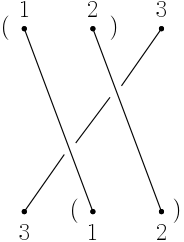
\includegraphics[scale=0.6]{Imagenes/left}
\end{figure}
This morphism is nothing more than $d_1x$, so it is mapped via $\phi$ to $d^1\exp(t_{12}/2)$. On the other hand, by composition it can be expressed in several steps, performing one crossing or chaging the parenthesizing on each step as follows

\begin{figure}[h!]
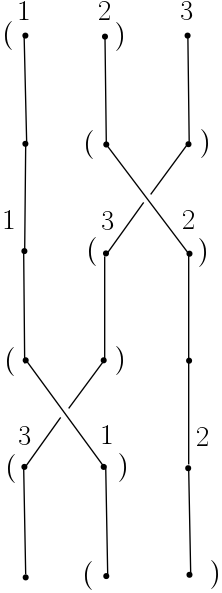
\includegraphics[scale=0.6]{Imagenes/right}
\end{figure}

This is the morphism obtained by the product $i\cdot d_0x\cdot (132)i^{-1}\cdot (13)d_3x\cdot (312)i$. This should be sent to $\Phi\cdot d^0\exp(t_{12}/2)\cdot (132)\Phi^{-1}\cdot (132)d^3\exp(t_{12}/2)\cdot (312)\Phi$. By definition of the $d^i$'s, we have $d^0\exp(t_{12}/2)=\exp(t_{23}/2)$ and $(132)d^3\exp(t_{12}/2)=\exp(t_{13}/2)$, so the morphism is mapped to $$\Phi\cdot \exp(t_{23}/2)\cdot (132)\Phi^{-1}\cdot (132)\exp(t_{13}/2)\cdot (312)\Phi,$$ which is equal to $d^1\exp(t_{12}/2)$ by the hexagon axiom.

Then, the map $\phi$ produces a map of operads $C_\star(PaB_*)=C_\star^\Q(\Q(PaB_*))\to C_\star(O_A(*))$.
%C_* ya era sobre Q, y hacerlo sobre PaB_* en realidad era sobre la realización del nervio, así que es linearizar al final. Lo otro es linearizar primero y luego coger el nervio para el caso lineal
It is well known that the homology operad of $C_\star(PaB_*)$ is $e_2$ because $PaB_*$ induces a little disks operad as we saw section in \ref{pab}. One checks that $\phi$ is a quasi-isomorphism for $*=2$ by an argument of dimension similar to the one in the proof of \ref{4.1}: it induces a surjective homomorphism (it sends generators to generators) between spaces of the same dimension. Hence it is a quasi-isomorphism of operads (since
$e_2$ is generated by $e_2(2)$). By Proposition \ref{4.1}, $h$ is a quasi-isomorphism. Thus, the
chain operad $C_*(PaB_*)$ is equivalent to $e_2$.



%DEBERÍA ESCRIBIR EN ALGÚN LADO LOS ESQUEMAS DE LAS DEMOSTRACIONES, LA GRANDE, LA DE LA FORMALDIAD, Y SI HAGO LA DE $G_\infty\to G$ TAMBIÉN
\end{document}
